 \documentclass[xcolor=dvipsnames,table]{beamer}

\usepackage{latexsym}
\usepackage[utf8]{inputenc}
\usepackage[brazil]{babel}
\usepackage{amssymb}
\usepackage{amsmath}
\usepackage{stmaryrd}
\usepackage{fancybox}
\usepackage{datetime}
\usepackage[T1]{fontenc}
\usepackage{graphicx}
\usepackage{graphics}
\usepackage{url}
\usepackage{algorithmic}
\usepackage{algorithm}
\usepackage{acronym}
\usepackage{array}

\usepackage{enumitem}

\newtheorem{definicao}{Definio}
\newcommand{\tab}{\hspace*{2em}}

\mode<presentation>
{
  \definecolor{colortexto}{RGB}{0,0,0}
 
  \setbeamertemplate{background canvas}[vertical shading][ bottom=white!10,top=white!10]
  \setbeamercolor{normal text}{fg=colortexto} 

  \usetheme{Warsaw}
}

\title{Abordagem Tradicional}  

\author{
  Esdras Lins Bispo Jr. \\ \url{bispojr@ufj.edu.br}
  } 
 \institute{
  Tópicos em Informática e Educação \\Bacharelado em Ciência da Computação}
\date{\textbf{01 de abril de 2026} }

\logo{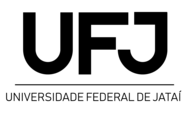
\includegraphics[width=1.5cm]{images/ufjJataiLogo.png}}

\begin{document}

	\begin{frame}
		\titlepage
	\end{frame}

	\AtBeginSection{
		\begin{frame}{Sumário}%[allowframebreaks]{Sumário}
    		\tableofcontents[currentsection]
    		%\tableofcontents[currentsection, hideothersubsections]
		\end{frame}
	}

	\begin{frame}{Plano de Aula}
		\tableofcontents
		%\tableofcontents[hideallsubsections]
	\end{frame}
	
	\section{Instrução pelos Colegas}

        \begin{frame}{Pesquisa 004}
		\begin{block}{[P004]}
			Como foi a leitura do estudo prévio?
		\end{block}
		\begin{enumerate}[label=(\Alph*)]
			\item Boa leitura
			\item Leitura razoável
			\item Difícil de ler
			\item Não consegui ler
		\end{enumerate}
	\end{frame}

\begin{frame}{Questão 018}
		\begin{block}{[Q018]}
		 São características gerais da abordagem tradicional, \underline{\bf exceto}:
		\end{block}
		\begin{enumerate}[label=(\Alph*)]
			\item Não se fundamenta em teorias empiricamente validadas.
			\item É uma prática educacional que persiste no tempo.
			\item Privilegia os processos de de participação ativa dos alunos.
			\item Serve como quadro referencial para outras abordagens. 
		\end{enumerate}
	\end{frame}

\begin{frame}{Questão 019}
		\begin{block}{[Q019]}
		 São condizentes com a percepção de ser humano da abordagem tradicional, \underline{\bf exceto}:
		\end{block}
		\begin{enumerate}[label=(\Alph*)]
			\item Há uma ênfase bastante forte à dimensão interna do aluno.
			\item É um receptor passivo, necessitando adquirir informações.
			\item O adulto é considerado como um homem acabado, ``pronto''.
			\item O aluno é considerado um ``adulto em miniatura'', que precisa ser atualizado. 
		\end{enumerate}
	\end{frame}

\begin{frame}{Questão 020}
		\begin{block}{[Q020]}
		 São condizentes com a concepção de mundo da abordagem tradicional, \underline{\bf exceto}:
		\end{block}
		\begin{enumerate}[label=(\Alph*)]
			\item O mundo é externo ao indivíduo.
			\item A posse do conhecimento sobre o mundo é realizada por meio da transmissão de especialistas para os estudantes.
			\item Instituições como escola, família e igreja transmitem a realidade para as pessoas.
			\item O conhecimento acumulado sobre o mundo é confrontado pelo aluno a partir de sua compreensão e construção.
		\end{enumerate}
	\end{frame}

\begin{frame}{Questão 021}
		\begin{block}{[Q021]}
		 São percepções sobre a sociedade e cultura da abordagem tradicional, \underline{\bf exceto}:
		\end{block}
		\begin{enumerate}[label=(\Alph*)]
			\item A trajetória da educação formal é definida por meio de níveis culturais.
			\item Enfatiza uma visão mais cooperativa do processo educacional.
			\item A reprovação do aluno é um indicativo da inadequação dele àquele nível cultural.
			\item Os diplomas e certificados são utilizados como instrumentos de hierarquização social.
		\end{enumerate}
	\end{frame}

    \begin{frame}{Questão 022}
		\begin{block}{[Q022]}
		 É condizente em relação à compreensão sobre o conhecimento na abordagem tradicional, \underline{\bf exceto}:
		\end{block}
		\begin{enumerate}[label=(\Alph*)]
			\item O estudante deve elaborar o conhecimento a partir de suas experiências anteriores.
			\item A inteligência como a faculdade de armazenar e acumular informações.
			\item O estudante deve incorporar informações sobre o mundo de forma gradativa.
			\item O passado é apresentado como modelo a ser imitado e como lição para o futuro.
		\end{enumerate}
	\end{frame}

\section{Próxima Aula}
\begin{frame}{Próxima Aula}
    \begin{block}{Apresentação}
        \begin{itemize}
            \item Tipos de Projetos em Informática e Educação (I\&E).  
        \end{itemize}
    \end{block}
\end{frame}
	
	\begin{frame}
		\titlepage
	\end{frame}
	
\end{document}